\documentclass[tikz, margin=0mm]{standalone}
\usepackage[utf8]{inputenc}
\usepackage{tikz}
\definecolor{white}{RGB}{255,255,255}
\usetikzlibrary{backgrounds}
\usepackage{tikz-qtree}
\usepackage{tikzscale}
\usetikzlibrary{arrows,automata,positioning,calc,snakes,decorations.pathmorphing}
\usepackage{libertine}

\begin{document}


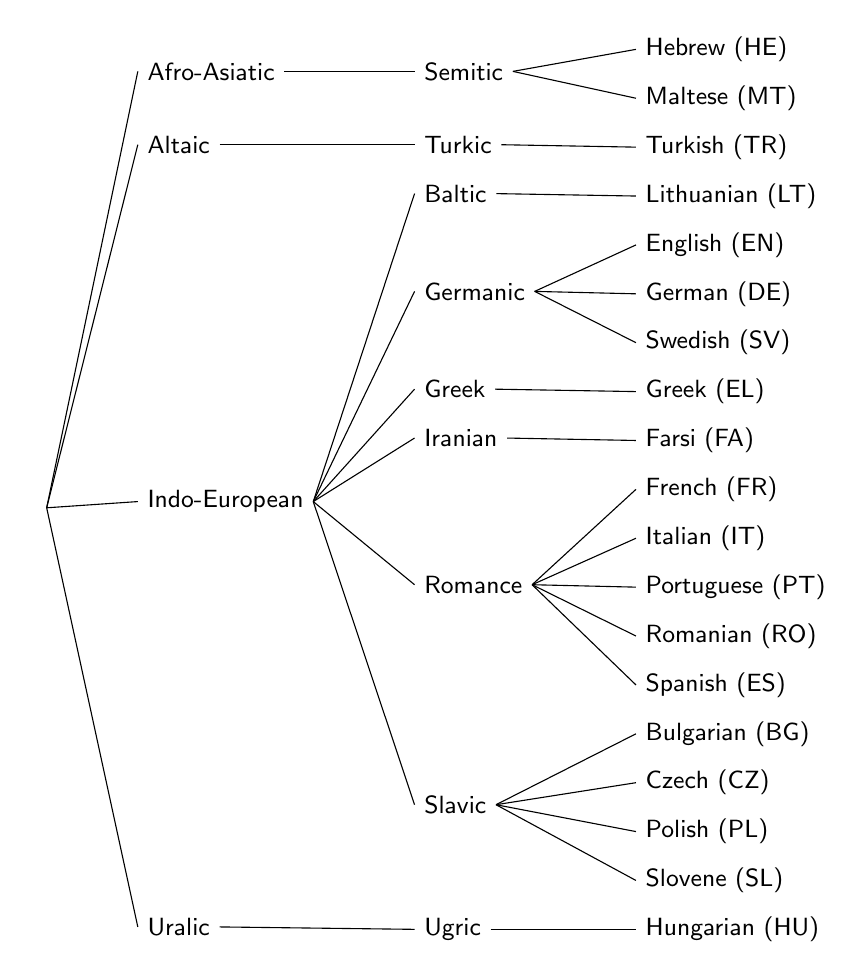
\begin{tikzpicture}[font=\sffamily\small]
\tikzset{grow'=right}
%\tikzset{level 1/.style={level distance=30pt}}
\tikzstyle{level 1}=[level distance=40pt]
\tikzstyle{level 2}=[level distance=100pt]
\tikzstyle{level 3}=[level distance=80pt]
%\tikzset{level 2 onwards/.style={level distance=80pt}}%\tikzset{execute at begin node=\strut}
\tikzset{every tree node/.style={anchor=base west}}
\Tree 
[.{~}
[.Afro-Asiatic [.Semitic {Hebrew (HE)} {Maltese (MT)} ] ]
[.Altaic [.Turkic {Turkish (TR)} ] ]
[.Indo-European 
	[.Baltic {Lithuanian (LT)} ] 
	[.Germanic {English (EN)} {German (DE)} {Swedish (SV)} ] 
	[.Greek {Greek (EL)} ] 
	[.Iranian {Farsi (FA)} ] 
	[.Romance {French (FR)} {Italian (IT)} {Portuguese (PT)} {Romanian (RO)} {Spanish (ES)} ] 
	[.Slavic {Bulgarian (BG)} {Czech (CZ)} {Polish (PL)} {Slovene (SL)} ] 
]
[.Uralic [.Ugric {Hungarian (HU)} ] ] 
]
\end{tikzpicture}

\end{document}

